
\documentclass[10pt, twocolumn]{article}
\usepackage{amsmath}
\usepackage{siunitx}
\usepackage{graphicx, float}
\usepackage[plain]{algorithm}
\usepackage{lipsum}

\topmargin=-0.45in
\evensidemargin=0in
\oddsidemargin=0in
\textwidth=6.5in
\textheight=9.0in
\headsep=0.25in


\title{Group Design Project: Formal Report}
\author{Alex Booth}



\begin{document}
    \maketitle

    \section{Introduction}
        \lipsum
    \section{Background and Theory Basis}
        \subsection{Introduction}
            For a building to function as both a music studio and as an educational facility, special considerations must be taken.
        \subsection{Educational facilities}
            Any building that facilitates or is used for educational purposes must comply to the education building regulations specified by the government.
            These specifications are laid out in Building Bulletin 93 (BB93): Acoustic design of schools - performance standards.
            The importance of acoustic considerations is given by the National Education Union: "Noise from adjacent rooms disrupts the learning process, especially during quiet reading times or test-taking"\cite{NEU}
            The NEU further states the importance of tuning the reverb time of a classroom environment such that the teacher can be heard clearly at any point the classroom, but also so that the conversation of students does not descend into cacophony.
            In BB93, a table of appropriate $L_{AEQ}$ values are given for various classrooms.
            In this context, only the music rooms and common rooms entries are relevant.
            \begin{figure*}\label{BB93}
                \centerline{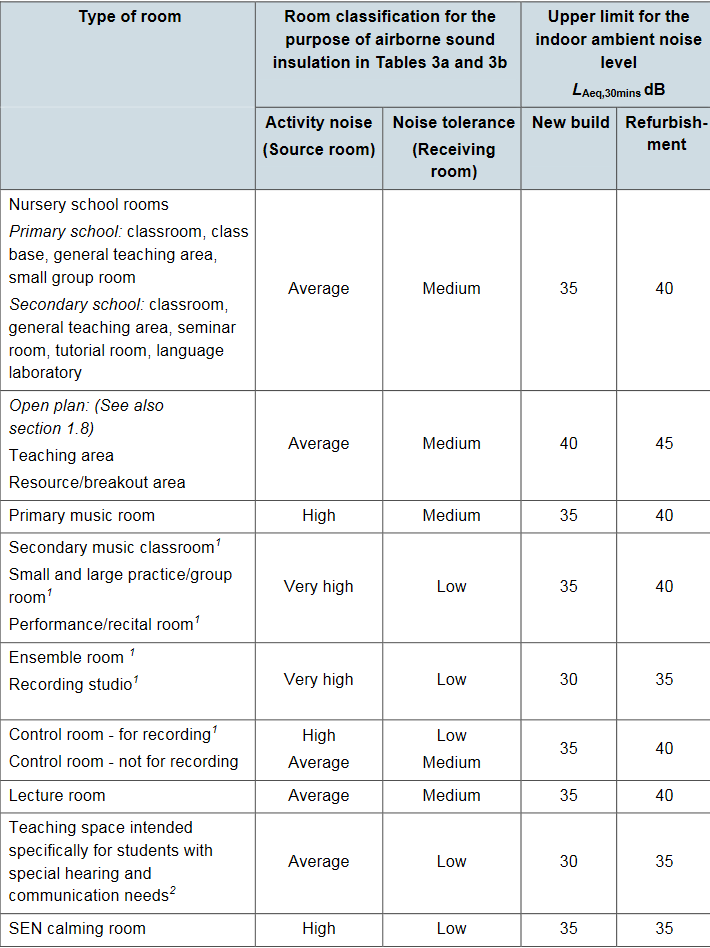
\includegraphics[scale = 0.8]{resources/BB93.png}}
                \caption{The tabulated $L_{AEQ}$ requirements of an educational environment}
                \centering
            \end{figure*}

        \subsection{Music facilities}
    \section{Building Layout}

        The floor plan of the envisioned building is illustrated in Fig.\ref{floorplan}:
        \begin{figure*}\label{floorplan}
            \centerline{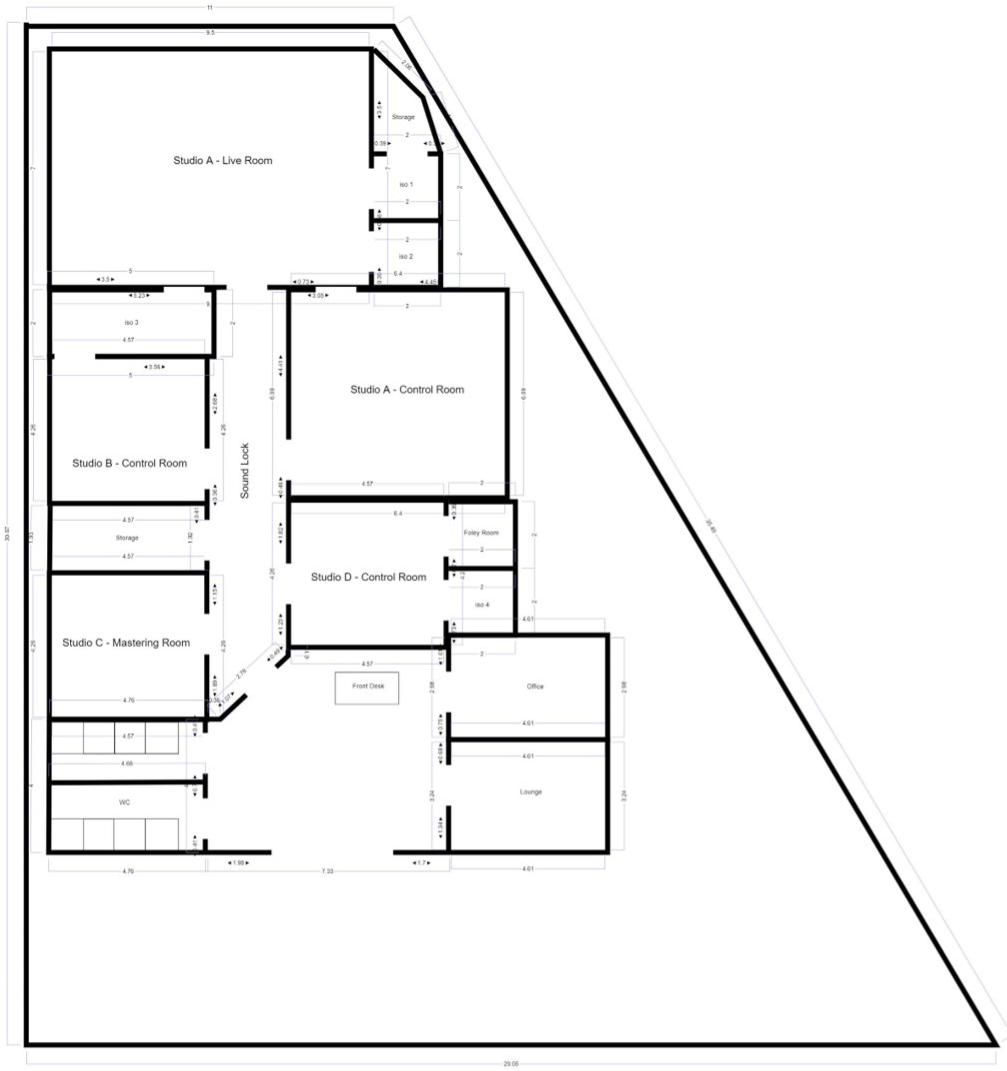
\includegraphics[scale = 0.8]{resources/floorplan.png}}
            \caption{The floor plan of the music educational facility}
            \centering
        \end{figure*}
    \section{Noise Criteria}
        \lipsum

    \section{Acoustic Parameters}
        \lipsum
    \section{Noise Insulation}
        \lipsum
    \section{Studio Layout}

    \section{Location case study}

    \bibliographystyle{plain}
    \bibliography{theBib}

\end{document}